\chapter{Preliminary Graph Theory}\label{ch:prelim}

First, let's define some basic concepts of graph theory, starting with the graph itself.

\section{Graphs}

A graph is an algebraic structure most commonly used to describe relationships between objects. There are many definitions of a graph. The most abstract definition of a graph is simply a set $V$ and a relation $R$ on $V$ denoting which elements of $V$ are connected. Graphs in general are \textit{directed}, if $R$ is symmetric, the graph is \textit{undirected}. For the purposes of this work we will be using a geometric definition and generally undirected graphs.

\begin{definition}
    An undirected graph is an ordered pair $G = (V, E)$, where $V$ is a set of \textit{vertices} and $E$ is a set of edges, i. e. a set of unordered pairs of vertices $\forall e \in E: ~ e = (u,v); u,v \in V$.
\end{definition}

\begin{definition}
    A \textit{path} in a graph $G$ from $v$ to $w$; $v,w \in V$ is a sequence of vertices $(u_1, u_2, \dots, u_n); ~ \{u_i ~|~ 1 \leq i \leq n\} \subseteq V$ such that $u_1 = v$, $u_n = w$ and $\{(u_i, u_{i+1}) ~|~ 1 \leq i \leq n-1\} \subseteq E$. A graph is \textit{connected} if there exists a path between every pair of vertices $v,w \in V; ~ v \neq w$.
\end{definition}

\begin{definition}
    A \textit{degree} $\Delta (v)$ of a vertex $v$ denotes how many edges are incident to this vertex. $\Delta(G)$ is the highest degree of any vertex in $G$.
\end{definition}

\begin{definition}
    A graph is \textit{k-regular} if the degree of each vertex is exactly $k$. A \textit{cubic graph} is a 3-regular graph.
\end{definition}

As an example, the $K_4$ graph is cubic.

\begin{figure}[h]
    \centering
        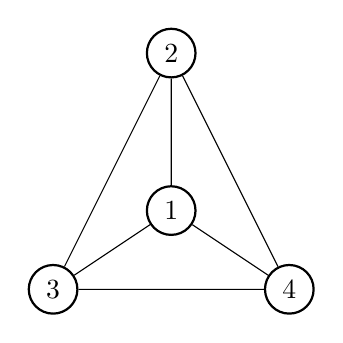
\begin{tikzpicture}
            \begin{scope}[every node/.style={circle,thick,draw}]
                \node (1) at (0,0) {1};
                \node (2) at (0,2) {2};
                \node (3) at (-1.5,-1) {3};
                \node (4) at (1.5,-1) {4};
            \end{scope}
            \draw (1) -- (2) -- (3) -- (4) -- (1) (2) -- (4) (1) -- (3);
        \end{tikzpicture}
\end{figure}

In general statements about graphs in later chapters, we are referring to unordered cubic graphs.

\subsection{Coloring}

When simple binary relationships between objects are not enough, weighted graphs and coloring offer a wider range of applications. Assigning colors to vertices or edges of graphs makes classifications of these objects possible.

\begin{definition}
    A vertex coloring $\phi(G)$ of a graph $G$ is a mapping from the vertex set of $G$ to a set of colors $C$. An edge coloring $\gamma(G)$ of a graph $G$ is a mapping from the edge set of $G$ to a set of colors $C$.
\end{definition}

\begin{definition}
    A \textit{proper vertex coloring} of $G$ is a vertex coloring such that no two neighboring vertices share a color. A \textit{proper edge coloring} is an edge coloring such that no two edges that share an endpoint have the same color. A proper coloring using $k$ colors is called a \textit{k-coloring}.
\end{definition}

As coloring in general is not very interesting, we will be considering only proper colorings henceforth. It is also important to define the set of "colors", especially when coloring signed graphs. Although actual colors tend to be a nice visualization of a coloring, it is more practical to use a subset of integers $C \subseteq \mathbb{Z}$.

The canonical coloring problem is to find the minimum number of colors required for a proper coloring. This number is called the \textit{chromatic number} for vertex colorings and \textit{chromatic index} for edge colorings. Determining the chromatic number and index is useful in other areas of graph theory as well.

\begin{theorem}\label{th:bipartite}
    A graph is bipartite if and only if it has a proper vertex 2-coloring.
\end{theorem}

For regular unsigned graphs these numbers are known.

\begin{theorem}[Brooks]
    The chromatic number of a graph $G$ is $\Delta(G)$ for all graphs except complete graphs and cycles of odd length, where the chromatic number is $\Delta(G) + 1$.\cite{brooks}
\end{theorem}

\begin{theorem}[Vizing]
    The chromatic index of a graph $G$ is $\Delta(G)$ or $\Delta(G) + 1$.\todo{cite}
\end{theorem}

In other words, we can always color the edges of a graph using at most $\Delta(G) + 1$ colors where $\Delta(G)$ is the highest degree of any vertex in $G$. The lower bound $\Delta(G)$ is trivial; we need exactly $\Delta(G)$ colors at the highest degree vertex in $G$ to construct a proper coloring. The Vizing theorem\todo{CITE VIZING THEOREM} proves the upper bound using Kempe chains.

\section{Signed graphs}

A signed graph is a graph in which each edge has either a positive or a negative sign. There are multiple definitions of a signed graph but for our purposes a sign function is most practical.

\begin{definition}
    A \textit{signed graph} $\Gamma = (G, \sigma)$ consists of a \textit{base graph} $G$ and a \textit{sign function} $\sigma : E(G) \rightarrow \{+,-\}$ that assigns a sign to each edge of $G$.
\end{definition}

\begin{figure}[h]
    \centering
        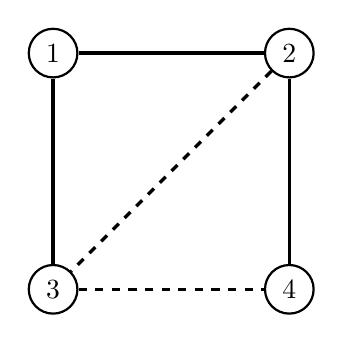
\begin{tikzpicture}
            \begin{scope}[every node/.style={circle,thick,draw}]
                \node (1) at (0,0) {1};
                \node (2) at (3,0) {2};
                \node (3) at (0,-3) {3};
                \node (4) at (3,-3) {4};
            \end{scope}
            \begin{scope}[every edge/.style={draw,very thick}]
                \path
                    (1) edge (2)
                    (2) edge [dashed] (3)
                    (3) edge (1)
                    (2) edge (4)
                    (3) edge [dashed] (4);
            \end{scope}
        \end{tikzpicture}
    \caption[Example of a signed graph]{Example of a signed graph. Dashed lines indicate negative edges, solid lines positive edges.}
\end{figure}

A fundamental concept in the signed graphs theory is \textit{balance}. The sign of a path is the product of the signs of its edges. A path is positive if and only if there is an even number of negative edges on it. A cycle is balanced if it is positive and a signed graph is balanced if each cycle in it is balanced\cite{harary}.

\begin{theorem}[Harary]\label{th:harary}
    A signed graph is balanced if and only if
    \begin{enumerate}
        \item for every pair of vertices, all paths between these vertices have the same sign
        \item the vertices can be divided into two subsets (possibly empty) such that each edge with both ends in the same subset is positive and each edge with ends in different subsets is negative
    \end{enumerate}

    This is the generalization of the earlier mentioned bipartite graph theorem.\todo{reference?}
\end{theorem}

The proof uses the method of \textit{switching}. Switching a vertex of a signed graph reverses the sign of each edge incident to it. More generally, switching a signed graph reverses the sign of each edge between a vertex subset and its complement.

\begin{figure}[h]\label{fig:switching}
    \centering
        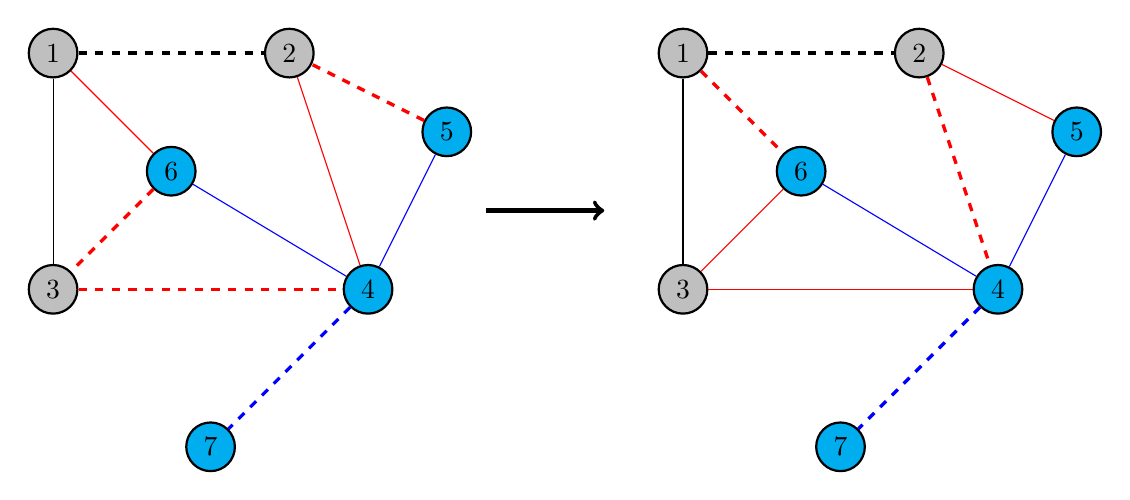
\begin{tikzpicture}
            \begin{scope}[every node/.style={circle,thick,draw,fill=lightgray}]
                \node (1) at (0,0) {1};
                \node (2) at (3,0) {2};
                \node (3) at (0,-3) {3};
            \end{scope}
            \begin{scope}[every node/.style={circle,thick,draw,fill=cyan}]
                \node (4) at (4,-3) {4};
                \node (5) at (5,-1) {5};
                \node (6) at (1.5,-1.5) {6};
                \node (7) at (2,-5) {7};
            \end{scope}
            \begin{scope}[every edge/.style={draw,dashed,very thick}]
                \path
                    (1) edge (2)
                    (3) edge [color=red] (4)
                    (4) edge [color=blue] (7)
                    (5) edge [color=red] (2)
                    (6) edge [color=red] (3);
            \end{scope}
            \begin{scope}[every every edge/.style={draw,very thick}]
                \path
                    (1) edge [color=red] (6)
                    (2) edge [color=red] (4)
                    (3) edge (1)
                    (4) edge [color=blue] (5)
                    (4) edge [color=blue] (6);
            \end{scope}

            \draw [ultra thick, ->] (5.5,-2) -- (7,-2);

            \begin{scope}[every node/.style={circle,thick,draw,fill=lightgray}]
                \node (11) at (8,0) {1};
                \node (21) at (11,0) {2};
                \node (31) at (8,-3) {3};
            \end{scope}
            \begin{scope}[every node/.style={circle,thick,draw,fill=cyan}]
                \node (41) at (12,-3) {4};
                \node (51) at (13,-1) {5};
                \node (61) at (9.5,-1.5) {6};
                \node (71) at (10,-5) {7};
            \end{scope}
            \begin{scope}[every edge/.style={draw,dashed,very thick}]
                \path
                    (21) edge [color=red] (41)
                    (11) edge [color=red] (61)
                    (11) edge (21)
                    (41) edge [color=blue] (71);
            \end{scope}
            \begin{scope}[every every edge/.style={draw,very thick}]
                \path
                    (31) edge (11)
                    (41) edge [color=blue] (51)
                    (41) edge [color=blue] (61)
                    (31) edge [color=red] (41)
                    (51) edge [color=red] (21)
                    (61) edge [color=red] (31);
            \end{scope}
        \end{tikzpicture}
    \caption[Example of a switching]{Example of a switching. Note that switching blue vertices and switching grey vertices results in the same transformation.}
\end{figure}

We can prove by induction that a signed graph can be switched to an all-positive graph if and only if it is balanced. Both conditions in Harary's theorem apply to all all-positive graphs and graphs that can be switched from an all-positive graph. Consequently, all balanced graphs are equivalent to an all-positive graph, which is an alternative definition of a positive graph. Similarly, we call a graph \textit{antibalanced} if it is equivalent to an all-negative graph, (all cycles of even length in and antibalanced graph are positive and cycles of odd length are negative).

\begin{definition}
    If a signed graph can be obtained from another signed graph by switching, they are considered \textit{equivalent}. For a single base graph, switching forms \textit{equivalence classes} of signed graphs. Within a single equivalence class all graphs can be switched to each other.
\end{definition}

It makes sense to study properties of signed graphs that behave consistently under switching. An example of such property is the sign of cycles. Switching a single vertex doesn't change the sign of cycles (cycles containing the vertex reverse signs for two edges resulting in the same product) and switching a set of vertices is equivalent to a sequence of one-vertex-switches (each edge within the set and within the complement gets reversed twice).

\subsection{Coloring}

The research in signed graph coloring was initiated by Zaslavsky\cite{zaslavsky-graphs} in the early 1980s and published in multiple seminary papers\cite{zaslavsky-invariants,zaslavsky-coloring,zaslavsky-colorful}.

\section{Motivation}

\say{In the study of various important and difficult problems in graph theory (such as the cycle double cover conjecture and the 5-flow conjecture), one encounters an interesting but somewhat mysterious variety of graphs called snarks. In spite of their simple definition [\dots] and over a century long investigation, their properties and structure are largely unknown.} --- Chladný, Škoviera \cite{skoviera-citat}

\todo{}
